\documentclass[10pt]{article}
\usepackage{babel}
\usepackage{hyperref}
% \usepackage{fullpage}
\usepackage[margin=0.6in]{geometry}
\usepackage[bottom]{footmisc}
\usepackage[export]{adjustbox}
\usepackage{wrapfig}
\usepackage{float}
\usepackage{hyperref}


\hypersetup{colorlinks=true, linkcolor=blue, filecolor=magenta, urlcolor=cyan}

%% Ingen innrykk ved nye avsnitt, sett avstand mellom avsnitt.
\setlength{\parindent}{0cm}
\setlength{\parskip}{.35\baselineskip}

\newlength{\cw}
\setlength{\cw}{2.0cm}
\newlength{\cwl}
\setlength{\cwl}{15.85cm}

\begin{document}
\begin{center}
\Large{Peder Ingmar Dahl}
\end{center}

%% Date
%% \today

%% Passbilde

\begin{wrapfigure}{r}{0.17\textwidth}
  \begin{center}
    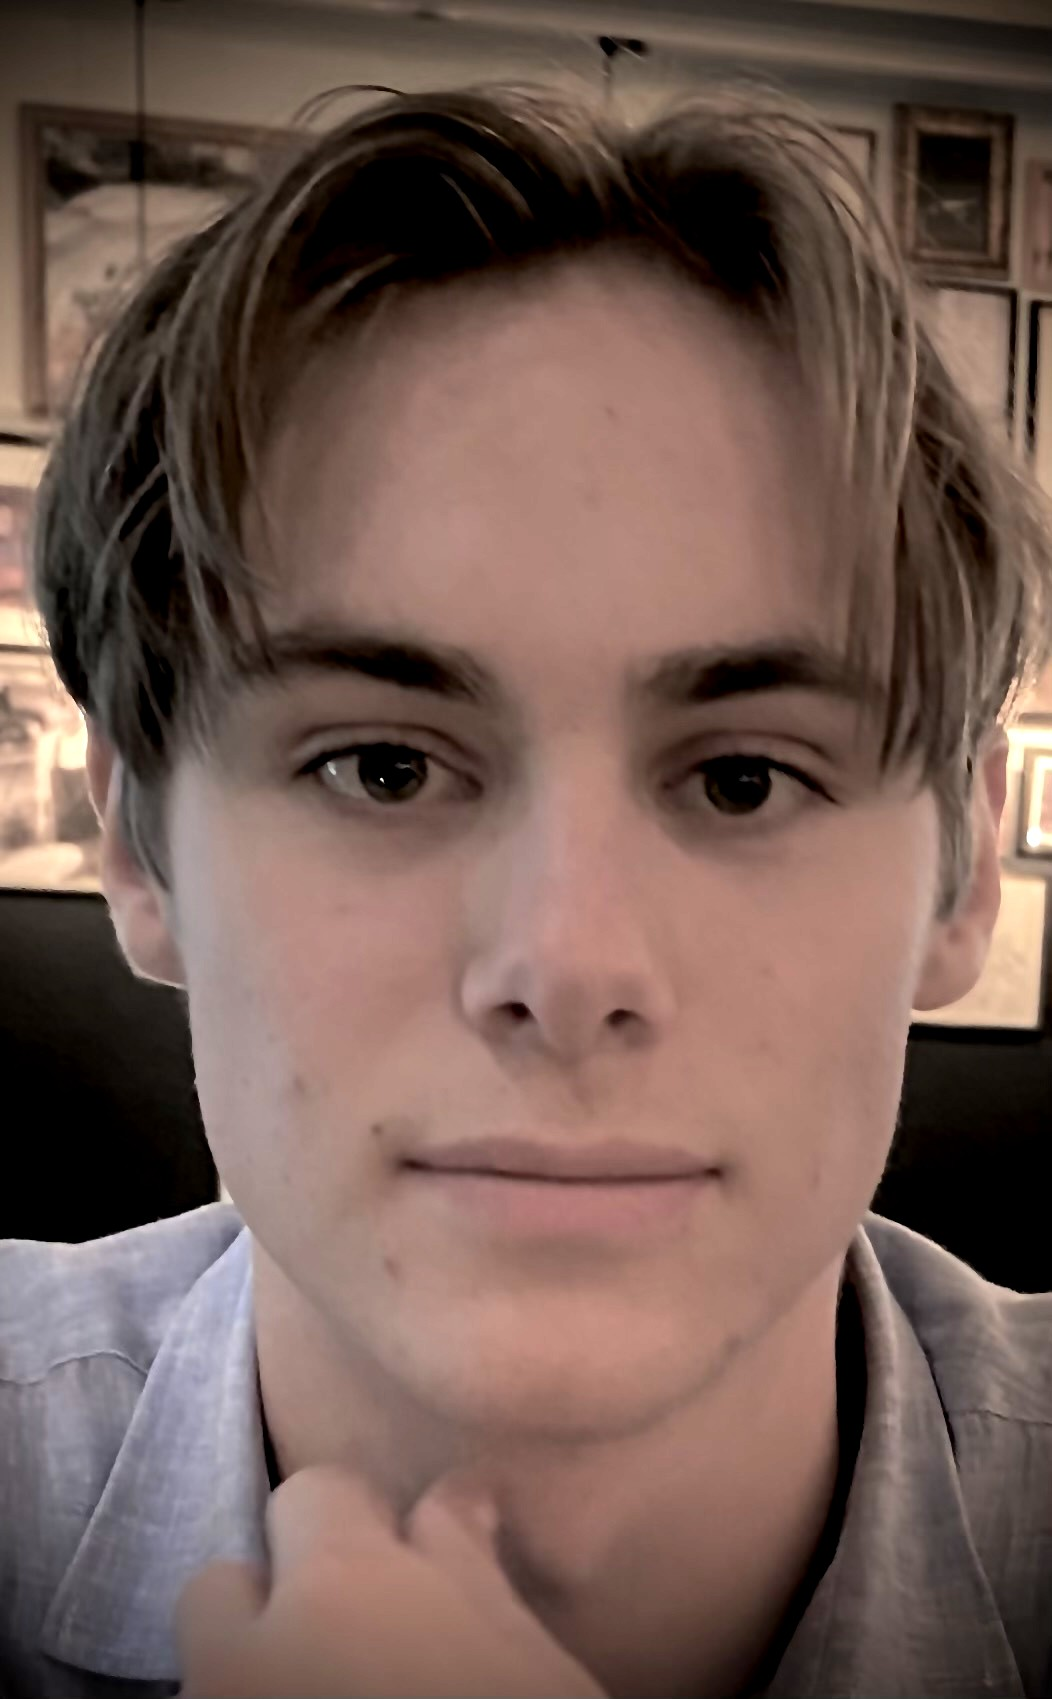
\includegraphics[width=0.15\textwidth]{Vedlegg/IMG_1433_mod.jpg}
  \end{center}
    %%\adjustimage{width=.2\textwidth, right}{Peder-passbilde-bw.png}
\end{wrapfigure}

\subsection*{}
\begin{tabular}{p{\cw} @{ }l p{\cwl}}
 & & \\ 
\end{tabular}
\vspace{0.2cm}

\subsection*{Personalia}
\begin{tabular}{p{\cw} @{:}l p{\cwl}}
Name & & Peder Ingmar Dahl \\
Address & & Askeladdveien 2, 0851 Oslo\\
Phone & & +47 91246056\\ 
E-mail & & piddi056@gmail.com \\
Born & & 14 March 2003 
\end{tabular}
\vspace{0.1cm}
\hrule
\vspace{0.1cm}

\subsection*{Education}
\begin{tabular}{p{\cw} @{:}l p{\cwl}}
  2022--current & & \textbf{NTNU}, Master's Programme Electronics Systems Design and Innovation. GPA: B \\
  2019--2022 & & \textbf{Nydalen VGS}. GPA: 5.87 \\ 
\end{tabular}
\vspace{0.1cm}
\hrule
\vspace{0.1cm}

\subsection*{Work experience}
 
\textbf{\href{https://www.newsec.no/}{Newsec} internships:}

\begin{tabular}{p{\cw} @{:}l p{\cwl}}
<<<<<<< Updated upstream
  2024 & & \textbf{Newsec:} Developed software for automated production of ESG reports for the real estate sector. I used Python and JavaScript for data collection and analysis, and HTML and CSS for the design of the report with subsequent automated generation of PDF reports for distribution. I used internal PostgreSQL databases and external APIs for data aggregation, while the front-end application was built using Python and the Streamlit library. Additionally, I gained experience in containerizing and hosting the application using Docker and GitHub Actions.  Although I worked on the project individually, it required collaboration and regular meetings across multiple departments at Newsec.
\end{tabular}

\textbf{\href{https://www.falkglobal.no/}{Falk} and \href{https://req.no/}{REQ Capital} summer internships:}

\begin{tabular}{p{\cw} @{:}l p{\cwl}}
  2023 & & \textbf{Falk:} Developed and implemented a client reporting tool, with the aim to increase efficiency and create an overview of deliverables and resource availability. The tool was designed for compliance, financial control, and regulatory reporting purposes. The reporting tool was built with Python, which automatically populated an internal Notion BI dashboard by utilizing internal databases and external public APIs for data aggregation.\\
  
  2022 & & \textbf{Falk and REQ Capital:} Coding in Python of a framework for scraping information from various APIs and the web to internal systems.
=======
  2024 & & \textbf{Newsec:} Developed and implemented an application for the automated production of client reports.
  The goal of the project was to automate basic real estate analysis with a focus on ESG (Environmental, Social, and Governance) factors.
  This involved integrating internal PostgreSQL databases and external APIs for data aggregation.
  I used Python and JavaScript for data analysis, and HTML and CSS for presenting the data in PDF reports.
  The frontend application was built using Python with the Streamlit library.
  Additionally, I gained experience in containerizing and hosting the application using Docker and GitHub Actions.
  Although I worked on the project individually, it required collaboration and regular meetings across multiple departments at Newsec.
  \\
\end{tabular}

\textbf{\href{https://www.falkglobal.no/}{Falk} and \href{https://req.no/}{REQ} summer internships:}

\begin{tabular}{p{\cw} @{:}l p{\cwl}}
  2023 & & \textbf{Falk:} Developed and implemented a client reporting tool, with the aim to increase efficiency and create an overview of deliverables and resource availability.
  The tool was designed for compliance, financial control, and regulatory reporting purposes. The reporting tool was built in Notion utilizing internal databases and external APIs for data aggregation.\\
  2022 & & \textbf{Falk and REQ:} Coding in Python of a framework for scraping information from various APIs and the web to internal systems.
>>>>>>> Stashed changes
\end{tabular}

\vspace{0.1cm}
\hrule
\vspace{0.1cm}

\subsection*{Engagements}
\begin{tabular}{p{\cw} @{:}l p{\cwl}}
<<<<<<< Updated upstream
  2023--current & & Serving on the board of directors of \textbf{\href{https://www.etdagen.no/}{Elektronikk \& Teknologidagene}} as IT Manager, responsible for web development. I have gained valuable experience in Git and GitHub, working with infrastructure designed for collaborative development, and managing a team of 5 developers. The position also requires proficiency in TypeScript, Vue 3, and Nuxt 3, among other technologies. The project is publicly available on \href{https://github.com/et-dagen}{GitHub} and the web pages are here \href{https://www.etdagen.no/}. 
=======
  2023--current & & Serving on the board of directors of \textbf{Elektronikk \& Teknologidagene} as IT Manager, responsible for web development.
  So far, I have gained valuable experience in Git and GitHub, working with infrastructure designed for collaborative development, and managing a team of 5 developers.
  The position also requires proficiency in TypeScript, Vue 3, and Nuxt 3, among other technologies.
  The project is publicly available on \href{https://github.com/et-dagen}{GitHub} and the web page is online at \href{https://www.etdagen.no/}{https://www.etdagen.no/}.
>>>>>>> Stashed changes
  \\
  2022--2024 & & \textbf{Sanctus Omega Broderskab}: Leader of the sports committee.\\
\end{tabular}
\vspace{0.1cm}
\hrule
\vspace{0.1cm}

\newpage

\subsection*{Other}
\textbf{Olympiads and competitions:}

\begin{tabular}{p{\cw} @{:}l p{\cwl}}
  2021--2022 & & Competed in the second round of the Norwegian informatics Olympiad. Placed 9.\\
  2021--2022 & & Competed in the finals of the Norwegian Informatics Olympiad.\\
  2021--2022 & & Competed in the Norwegian Mathematics Olympiad (Abelkonkurransen). Placed 28.\\
\end{tabular}

\textbf{Sports:}

\begin{tabular}{p{\cw} @{:}l p{\cwl}}
<<<<<<< Updated upstream
  2022-current & & Part of the NTNU Basketball team, playing the central Norway second division.\\
  2011-2022 & & Basketball at Bislet Basketball Club. \\
  2017-2018 & & Part of the \href{https://www.basket.no/landslag/u16-menn/}{U16 national basketball team}. \\
=======
  2022-current & & NTNU Basketball team, playing the central Norway second division.\\
  2011-2022 & & Bislet Basketball Club.\\
  2018 & & U16 national basketball team. \\
   & & Indoor climbing. \\
>>>>>>> Stashed changes
\end{tabular}
\vspace{0.1cm}
\hrule
\vspace{0.1cm}

\subsection*{Hobbies}
Basketball, climbing, coding. 

\end{document}
